\section{Versuchsbeschreibung}
\label{section:Versuchsbeschreibung}
Der Versuch wird an dem im Folgenden beschriebenen Aufbau durchgeführt.\\
Mittelpunkt des Prüfstandes ist im Windkanal des Labors platzierte Modellrotor, welcher in \autoref{fig:Fluegelfront}
zu sehen ist. Die Kenndaten des Rotors sind in \autoref{tab:Rotorkenndaten} zusammengefasst.
\begin{figure}[H]
    \centering
    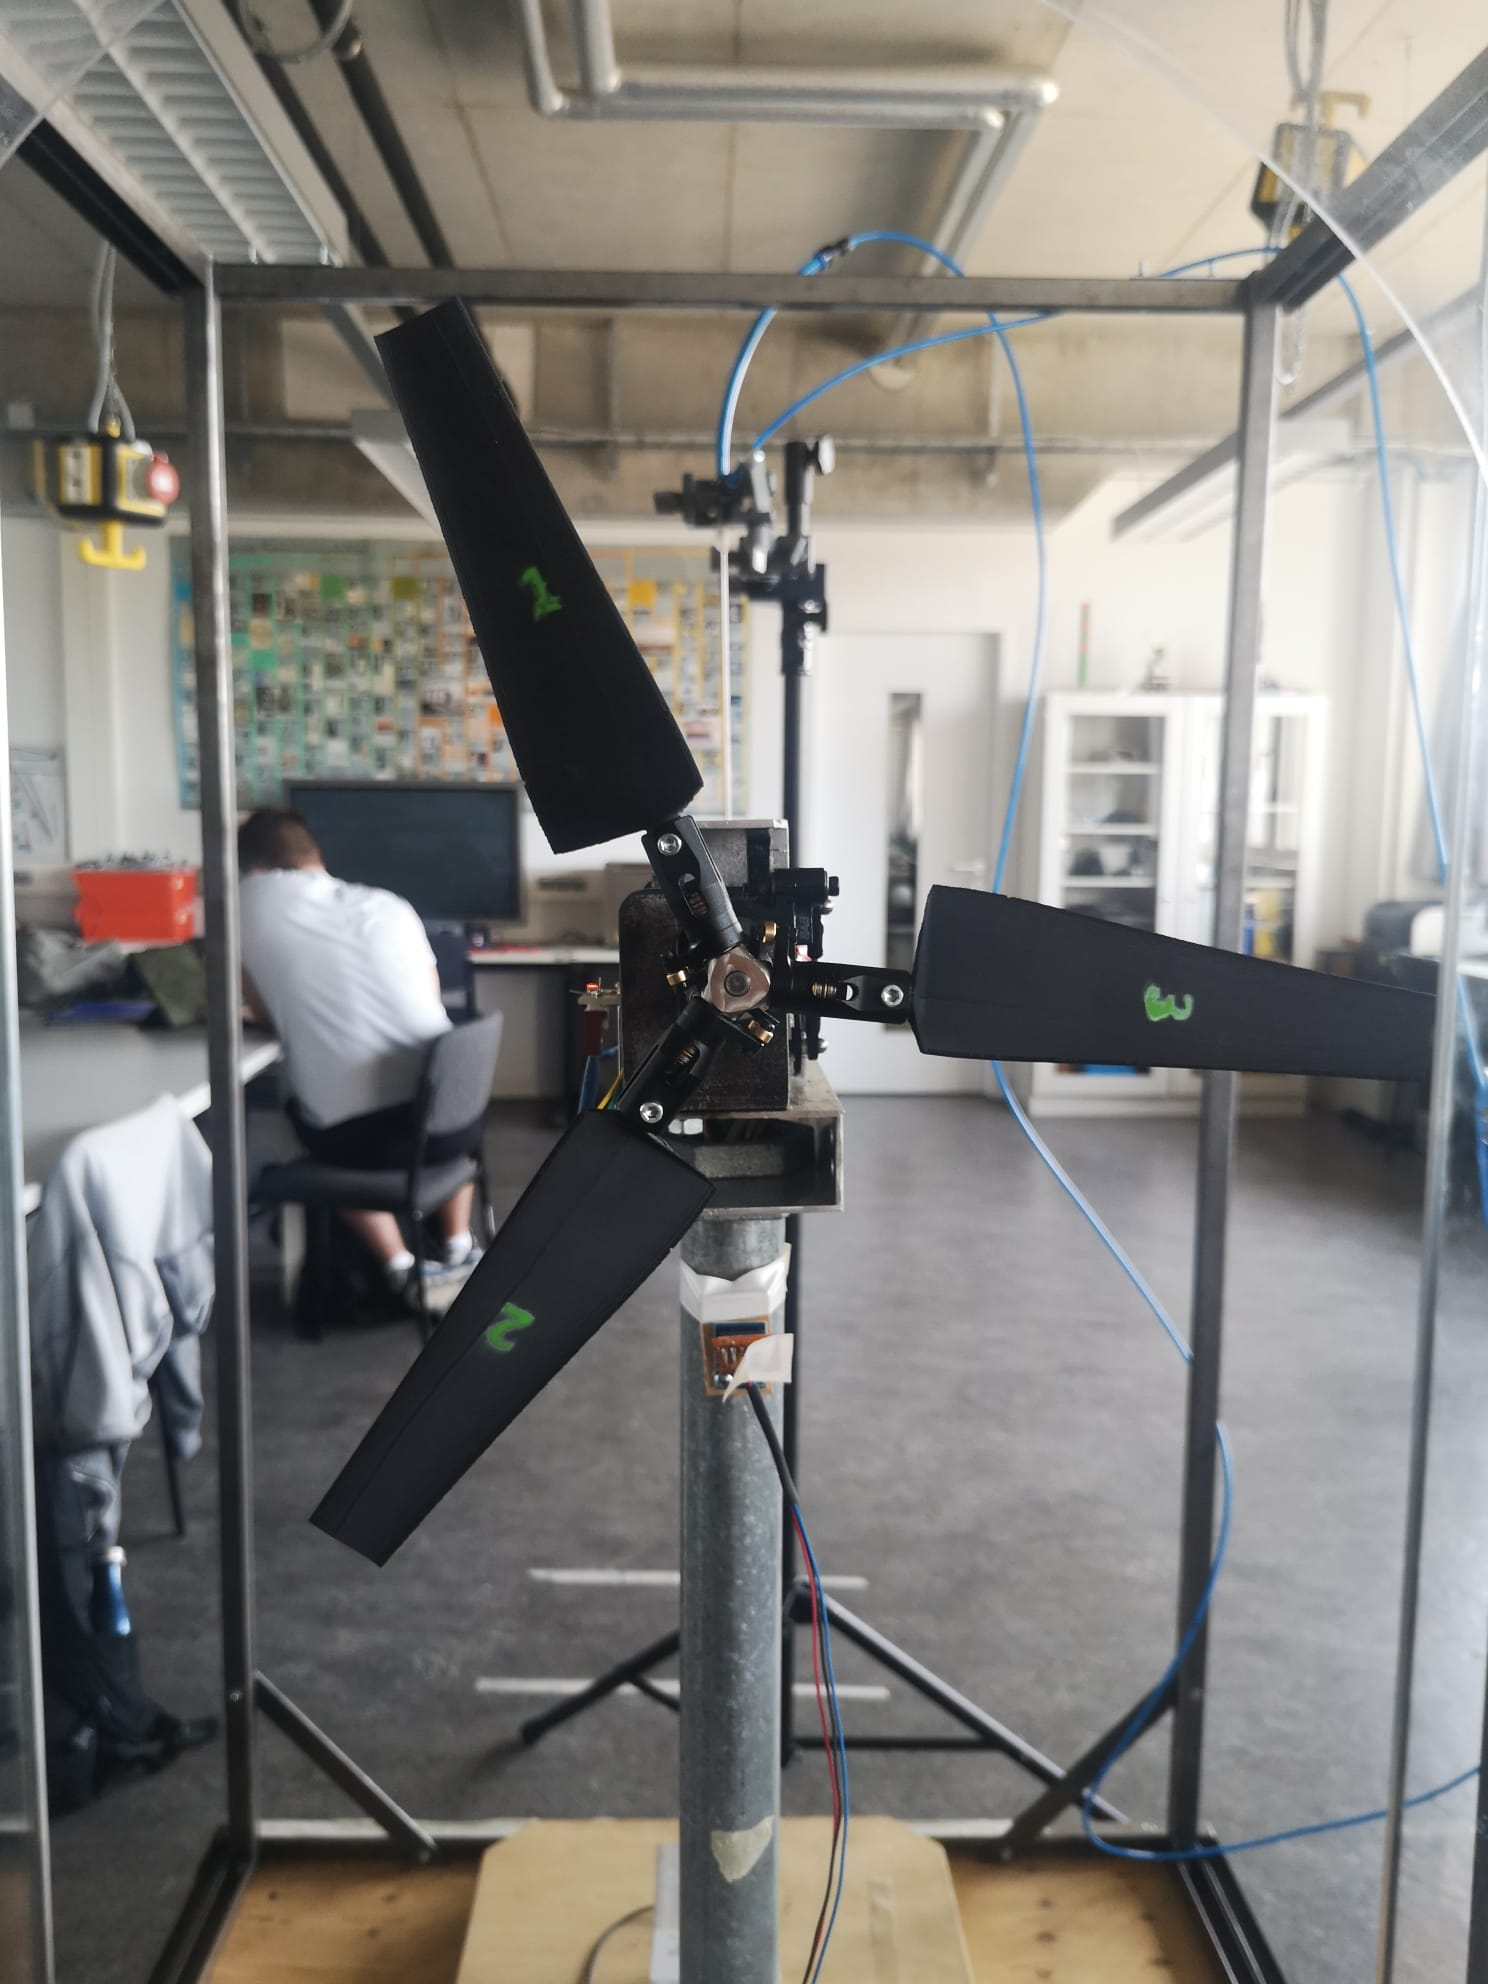
\includegraphics[width=0.75\textwidth]{Abbildungen/Fluegelfront.jpeg}
    \caption{Frontansicht der Rotorblätter des Versuchsaufbaus}
    \label{fig:Fluegelfront}
\end{figure}


\begin{table}[H]
    \centering
    \begin{tabular}{llll}
    \hline
                              & Symbol      & Wert & Einheit \\ \hline
    Rotordurchmesser          & $d_{Rotor}$ & 340  & mm      \\
    Auslegungsschnelllaufzahl & $\lambda_A$ & 3    &         \\
    Nabenhöhe                 & $h_N$       & 730  & mm      \\
    Hebelarm Schubmessung     & l           & 467  & mm      \\ \hline
    \multicolumn{4}{c}{Profil: Wortmann FX63}                \\ \hline
    \end{tabular}
    \caption{Kenndaten des Modellrotors}
    \label{tab:Rotorkenndaten}
    \end{table}
Der Rotor ist über eine Achse mit einem Gleichstrom-Generator gekoppelt und betriebt diesen.
Um alle zu betrachtenden Daten zu erhalten sind auf der Achse ein Reflektor für die Drehzahlmessung und an der Lagerung der Achse ein Drehmomentsensor verbaut.
Der gesamte Achsaufbau kann aus der Vogelperspektive in \autoref{fig:Achsaufsicht} zu sehen.\\
Die Einstellung des Pitchwinkels, welche für diesen Versuch entscheident ist, erfolgt über den Servomotor des Systems. Diese Einstellung erfolgt händisch über das in \autoref{fig:Laststeuerung} dargestellt Gerät.
Weitere Messeinrichtungen umfassen Prandtlsonden zur Ermittlung der Windgeschwindigkeiten, einen Sensor für alle weiteren Umgebungsbedingungen, sowie den \textit{Kraftsensor KD40S} der Firma \textit{ME-Meßsysteme GmbH}, mit welchem sich die Schubkraft ermitteln lässt.
Die in \autoref{fig:Messaufbau} zu sehenden Multimeter nehmen dann die Generatorspannung und den Generatorstrom auf.
    \begin{figure}[h!]
        \begin{minipage}[t]{\textwidth}
            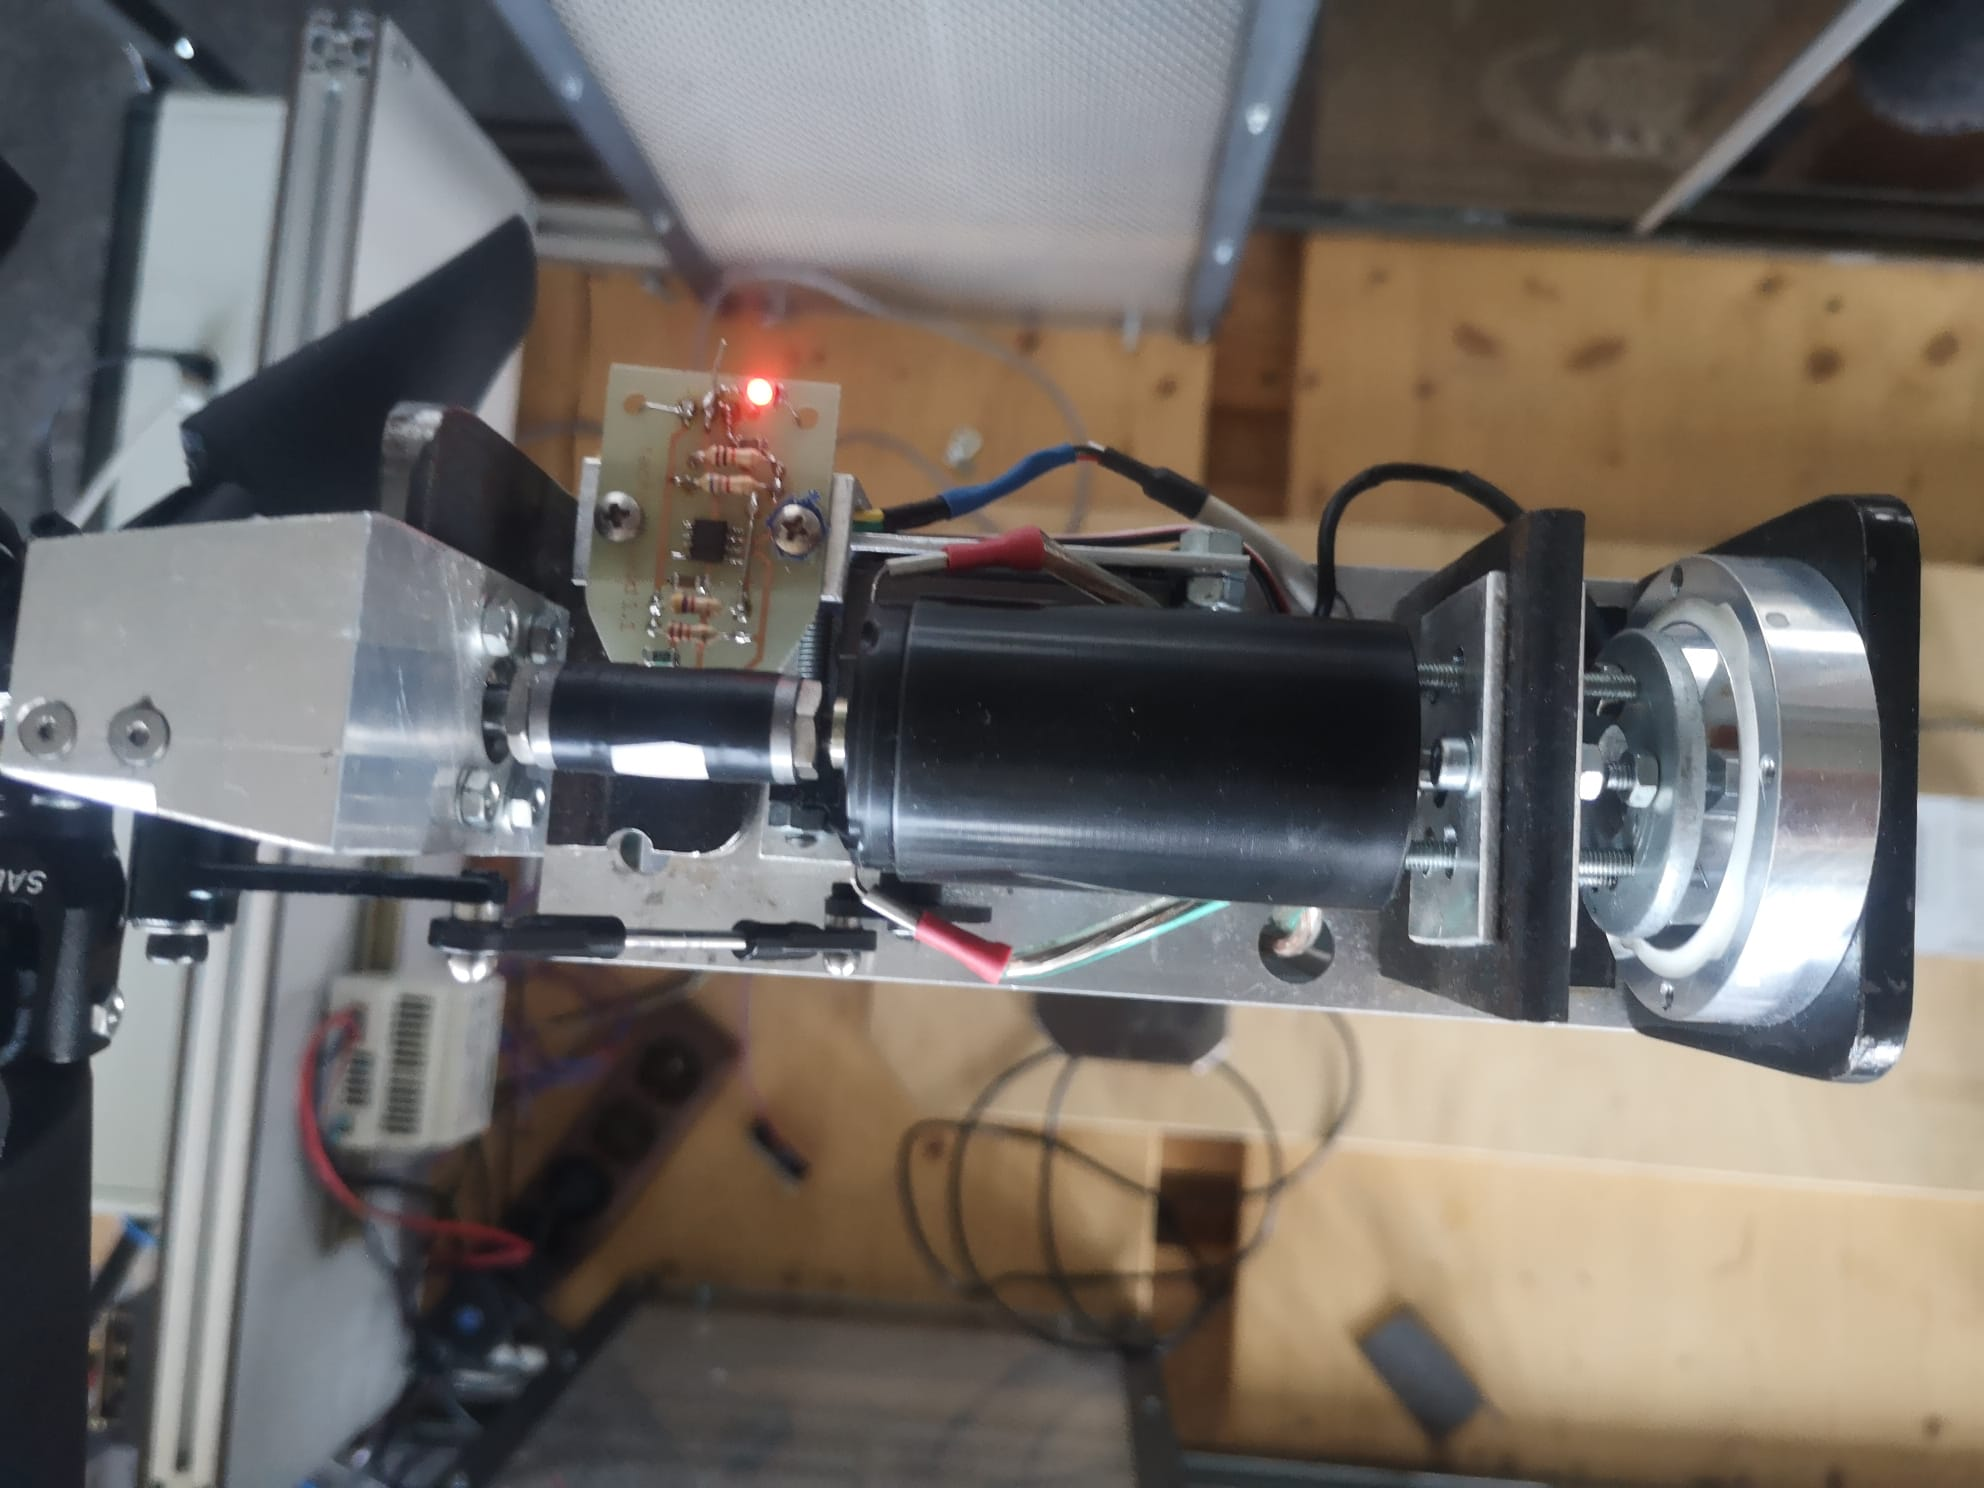
\includegraphics[width=\textwidth]{Abbildungen/Draufsicht Achse.jpeg}
            \caption{Draufsicht auf die Achse}
            \label{fig:Achsaufsicht}
        \end{minipage}
        \begin{minipage}[b]{0.5\textwidth}
            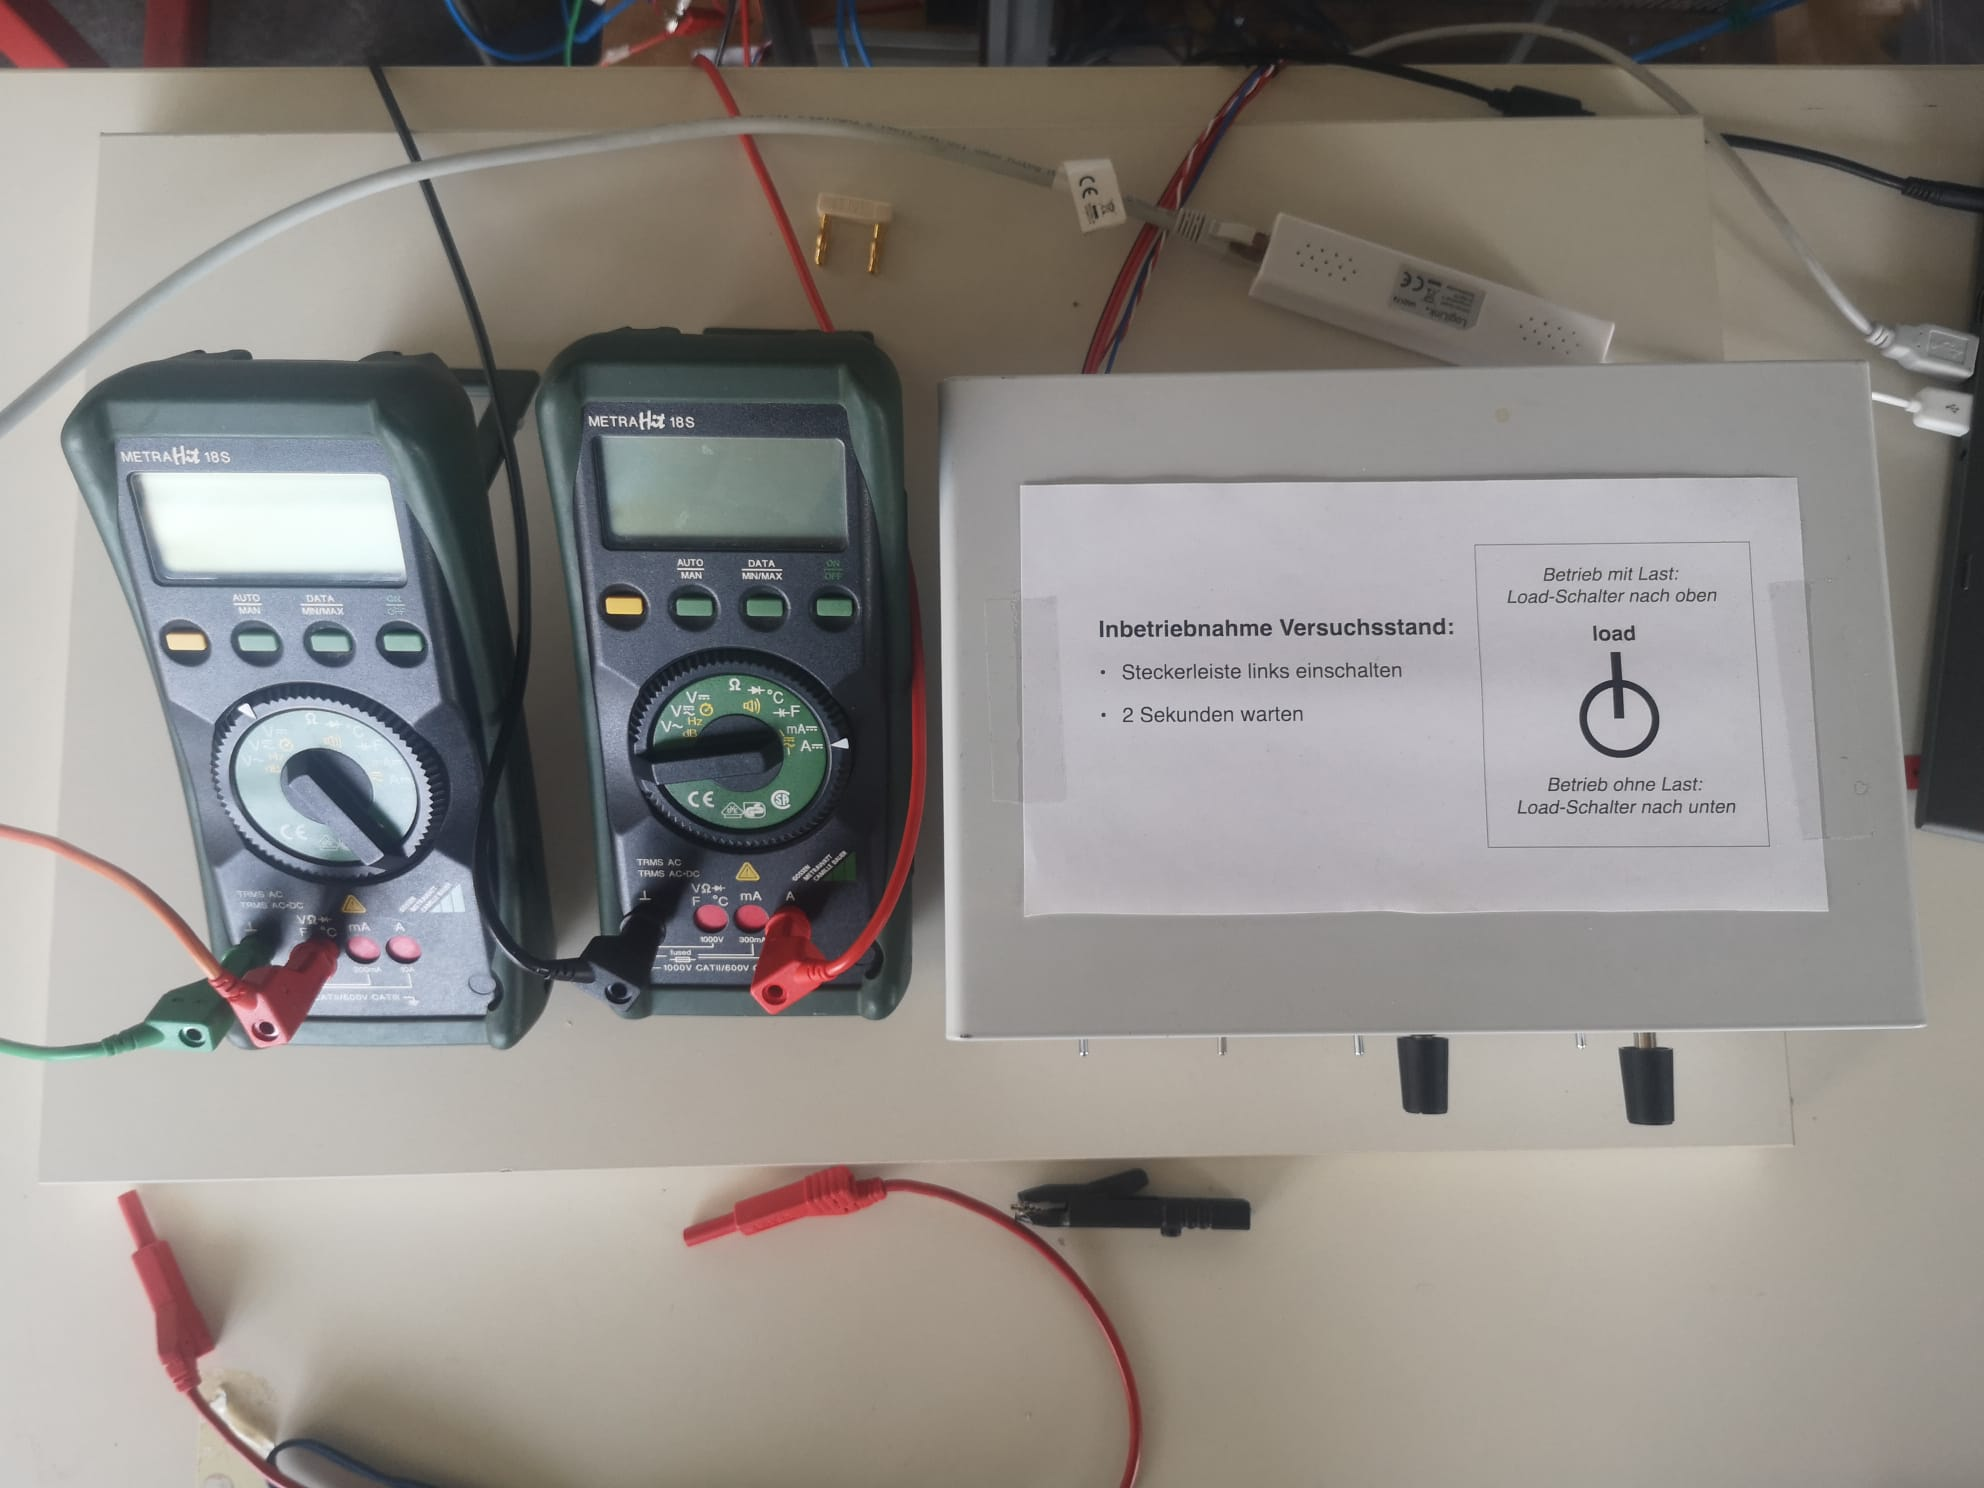
\includegraphics[width=\textwidth]{Abbildungen/Messaufbau.jpeg}
            \caption{Messaufbau Übersicht}
            \label{fig:Messaufbau}
        \end{minipage}
        \begin{minipage}[b]{0.5\textwidth}
            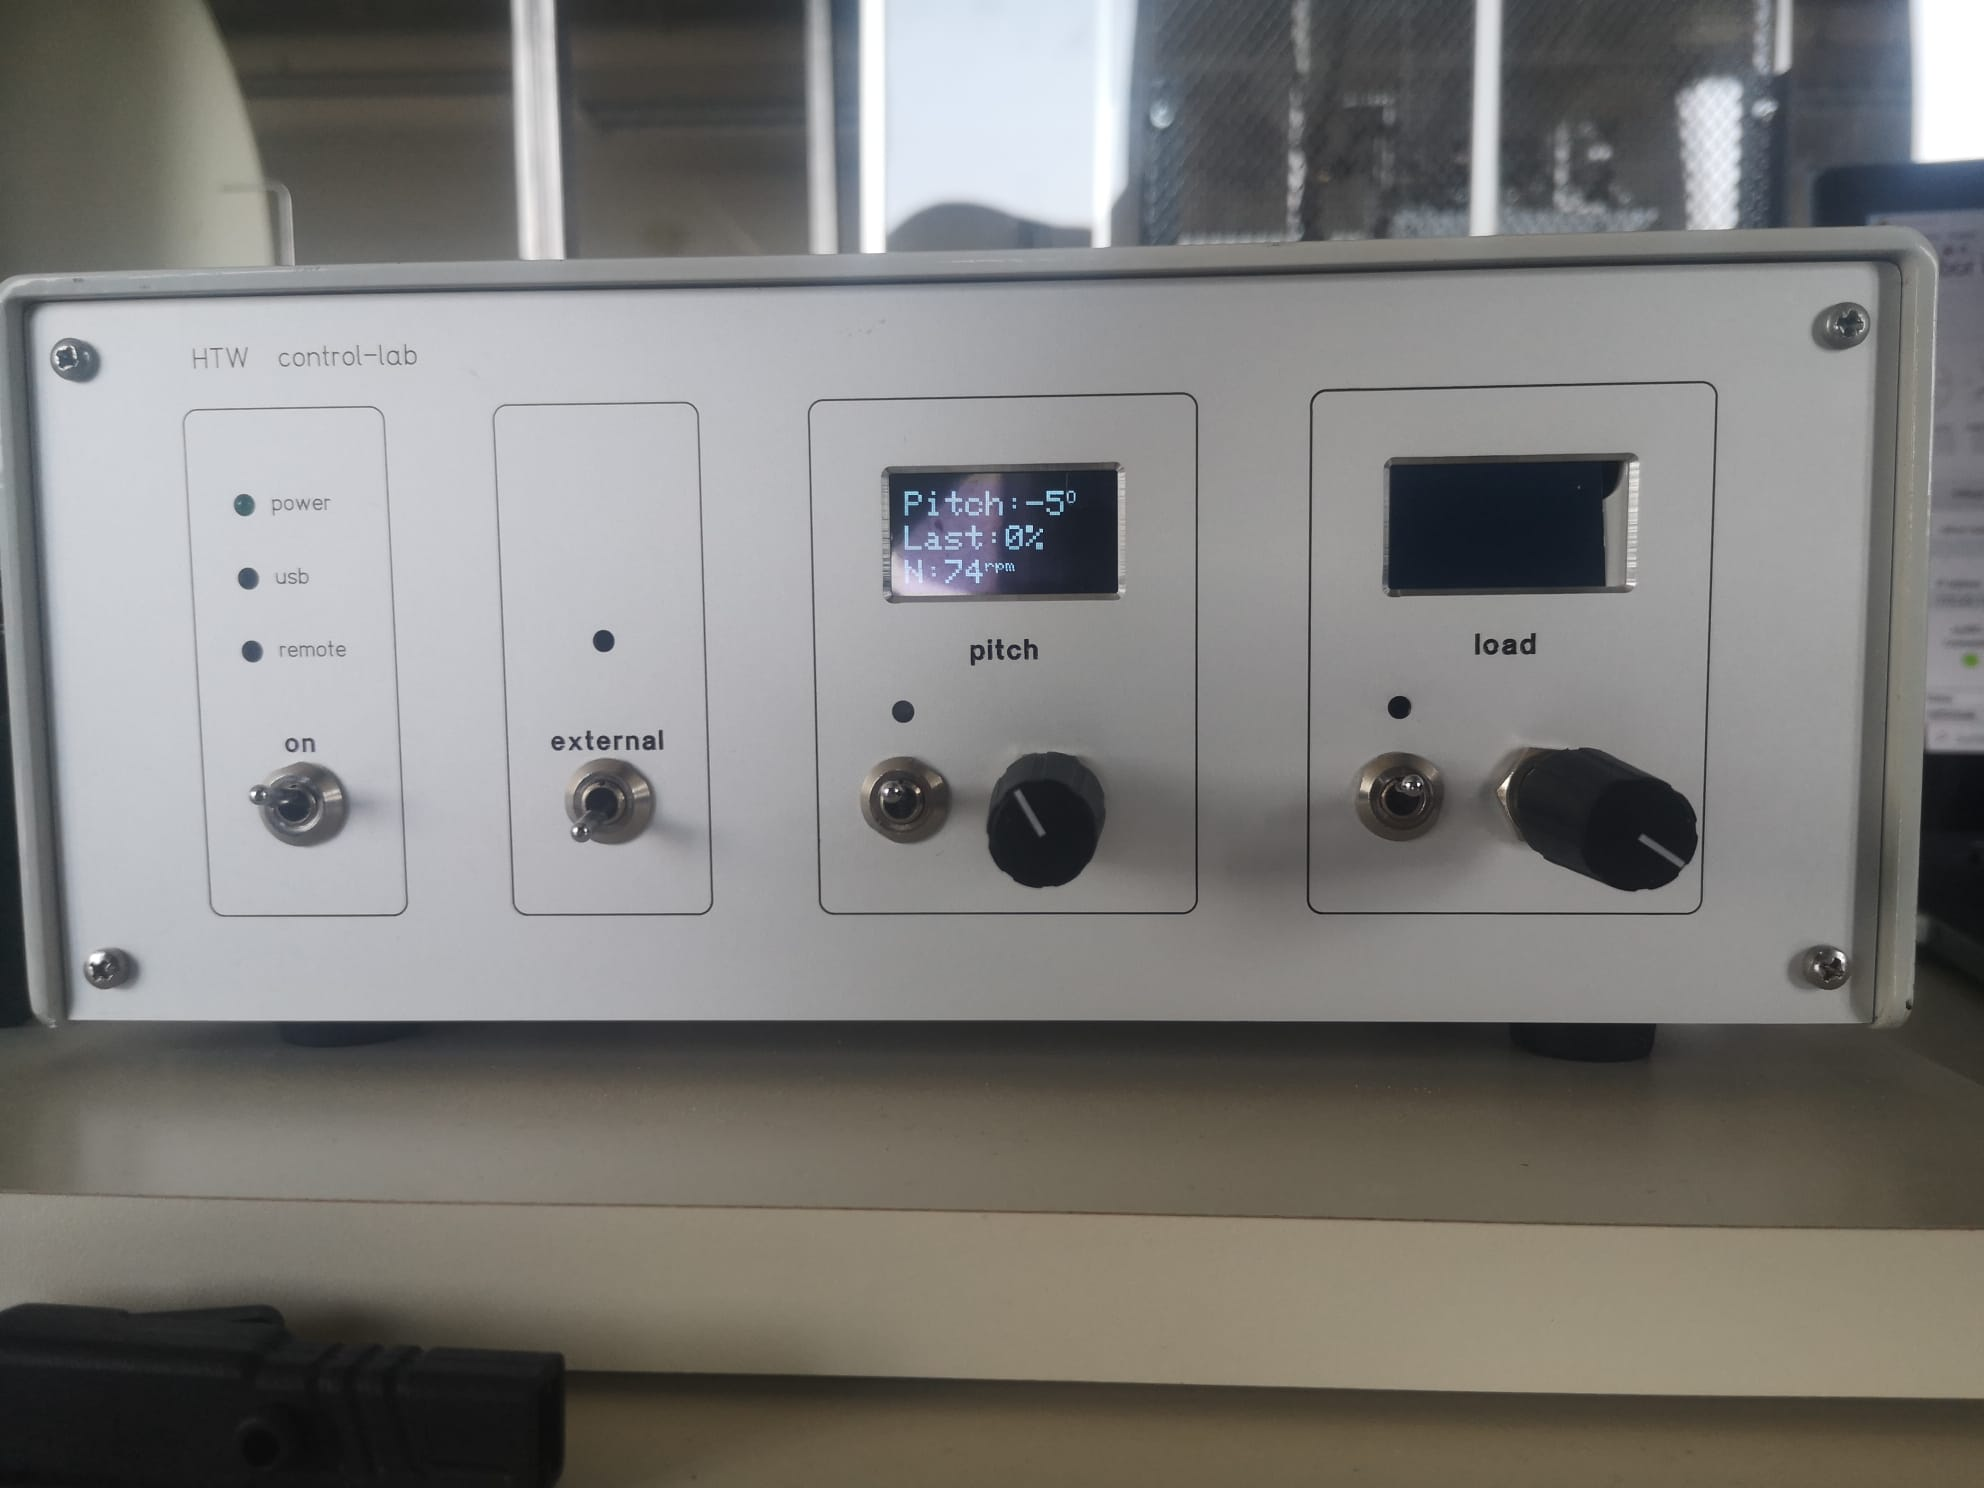
\includegraphics[width=\textwidth]{Abbildungen/Lastkontrolle.jpeg}
            \caption{Laststeuerung}
            \label{fig:Laststeuerung}
        \end{minipage}
    \end{figure}  